\documentclass{article}
\author{RustColeone}
\usepackage{amsmath}
\usepackage{amsfonts}
\usepackage{titling}
\usepackage{tikz}
\usepackage{hyperref}
%\setlength{\droptitle}{-12em}
\title{ECE, Signal Processing}

\begin{document}
\maketitle
\newpage
\tableofcontents
\newpage
\section{Sinusoidal Signals}
    \begin{enumerate}
        \item Sinusoidal signals are the basic building blocks in the theory of signals \& systems
        \item Arise as soutions to differential equations that through the laws of physics, describe common physical phenomena
    \end{enumerate}
    \subsection{Mathematical Formula}
    let a signal be $s(t)$, where t represents the time t of a given time, we have:
    \begin{align}
        s(t) &= A cos(2 \pi f_0 + \phi)
    \end{align}
    A linear function of time t, in which \textbf{A is the amplitude} that scales the cosine signal in y dimention, since
    \begin{align}
        -1 \leq cos(x) \leq 1 \text{for all } x, s(t) \in [-A, +A]
    \end{align}

    \textbf{$\phi$ is the phase in (rad)} that determines the time locations of the maxima and minima of $s(t)$\\

    eg: $\phi = 0 \implies s(0) = Acos(0) = A$, so $s(t)$ has a local maxima at 0

    if $\phi != 0 \implies s(0) = Acos(\phi)$, which is not necessary A\\
    
    Finding Maximum of the signal after t = 0
    \begin{align}
        Acos(2 \pi f_0 t + \phi) = A &\equiv cos(2 \pi f_0 t + \phi) = 1 \\
        2 \pi f_0 t + \phi &= 2 k pi \\
        t &= \frac{2 k pi - \phi}{2 \pi f_0}, \text{ } k \in \mathbb{Z}
    \end{align}

    \textbf{$f_0$ is the frequency in (Hz)}, determines the rate the signal oscillates
    
    \begin{align}
        \text{Period } T_0 &= \frac{1}{f_0}
    \end{align}
    \subsection{Periodic Signals}
    A periodic signal persists for an infinity amount of time, and will always output the same waveform in any integer multiples of periods

    \begin{align}
        s(t + T_0) &= s(t + T_0), \text{ for all t}
    \end{align}
    
    We can express $\phi$ as
    \begin{align}
        \phi &= 2 k \pi + \phi_0, k \in \mathbb{{z}}, \phi_0 \in [-\pi, \pi]
    \end{align}

    if $f_0 = 0$, for all values of $A cos(\phi)$ is a constant, hence a DC signal
    
    We can ecpress any arbitrary sinusoidal signal as a linear combination of the two pure sinusoidal signals:
    \begin{align}
        s(t) &= R \times cos(2 \pi f_0 t + \phi)\\
        s(t) &= A \times cos(s \pi f_0 t) + B \times sin(s \pi f_0 t)
    \end{align}
    where $A = R cos(\phi)$ and $B = R sin(\phi)$\\
    Using the formulae:
    \begin{align}
        sin(A \pm B) &\equiv sin(A)cos(B) \pm cos(A)sin(B)\\
        cos(A \pm B) &\equiv cos(A)cos(B) \mp sin(A)sin(B)\\
        tan(A \pm B) &\equiv \frac{tan(A) \pm tan(B)}{1 \mp Atan(B)}\\
        sin(3A) &\equiv 3sin(A) - 4sin^3(A)\\
        cos(3A) &\equiv 4cos^3(A) - 3cos(A)\\
        sin(P) + sin(Q) &\equiv  2 sin (\frac{1}{2}(P + Q)) cos (\frac{1}{2}(P - Q))\\
        sin(P) - sin(Q) &\equiv  2 cos (\frac{1}{2}(P + Q)) sin (\frac{1}{2}(P - Q))\\
        cos(P) + cos(Q) &\equiv  2 cos (\frac{1}{2}(P + Q)) cos (\frac{1}{2}(P - Q))\\
        cos(P) - cos(Q) &\equiv -2 sin (\frac{1}{2}(P + Q)) sin (\frac{1}{2}(P - Q))\\
    \end{align}

    \subsection{Harmonics}
    Lets say we have Harmonic Frequencies $f_k, k \in \mathbb{Z}$
    \begin{align}
        x_1(t) &= cos(2 \pi f_1 + \phi)\\
        x_2(t) &= cos(2 \pi f_2 + \phi)\\
        f_k &= k \times f_0, k \in \mathbb{Z}
    \end{align}
    Proof\:Any linear combination of sinusoidal signals of harmonics of some frequency $f_0$ is a periodic signal
    \begin{align}
        \text{For arbitrary } \{A_k\} \{\phi\}\\
        s(t) =& \sum_{k=1}^{N} A_k cos(2 \pi f_0t + \phi_k)\\
        s(t) =& \sum_{k=1}^{N} A_k cos(2 \pi f_0t + \phi_k)\\
        s(t + T_0) =& \sum_{k=1}^{N} A_k cos(2 \pi f_0 t + 2 \pi k + \phi_k)\\
        \text{hence: } s(t + T_0) =& s(t)\\
    \end{align}
    \subsection{Fourier Series}
    We can express any arbitrary periodic signal as a sum of harmonic sinusoids,
    let $x(t) = x(t + T_0)$ be a periodic signal with period $T_0$\\
    Then there exist coefficients:
    \begin{align}
        \{A_k\}_{k = 0}^{\infty}, \{B_k\}_{k = 0}^{\infty}\\
        x(t) &= \frac{A_0}{2} + \sum_{k=0}^{\infty}\left( A_k cos(2 \pi f_0 k t) + B_k sin(2 \pi f_0 k t)\right), \forall t
    \end{align}
    Calculating $\{A_k\}, \{B_k\}$ starting from $x(t)$
    It can be shown that:
    \begin{align}
        A_k &= \frac{2}{T_0} \int_{-0.5T_0}^{0.5T_0} x(t)cos(2\pi kt)dt\\
        B_k &= \frac{2}{T_0} \int_{-0.5T_0}^{0.5T_0} x(t)sin(2\pi kt)dt
    \end{align}

    Fourier synthesis is the reverse process of starting from $\{A_k\}_{k = 0}^{\infty}, \{B_k\}_{k = 0}^{\infty}$ and generates a periodic signal\\

    Equivalent Form:
    \begin{align}
        s(t) &= \frac{A_0}{2} \sum_{k=1}^{\infty} C_k cos(2 \pi f_0t + \phi_k)\\
        \text{where} \nonumber\\
        C_k &= \sqrt{A_k^2 + B_k^2} and \phi_k = tan^{-1}(\frac{B}{A})
    \end{align}

%    \begin{tikzpicture}
%        \draw[->] (-3,0) -- (4.2,0) node[right] {$x$};
%        \draw[->] (0,-3) -- (0,4.2) node[above] {$y$};
%        \foreach \ini [evaluate=\ini as \inieval using 2*\ini] in {0,...,1}
%        \draw[ultra thick,cyan] (\inieval,0) -- ++(0,3) -| (\inieval+1,0) -- (\inieval+2,0);
%        \draw[scale=0.5,domain=-3:3,smooth,variable=\y,red]  plot ({\y*\y},{\y});
%    \end{tikzpicture}

    \subsection{Spectrum}
    Fourier thyrm showed that all periodic signals can be written as an addictive linear combination of sinusoid signals

    The spectrum of a periodic signal is the collection of amplitude, frequency and phase information that allow us to represent the signal as a linear combination
    \begin{enumerate}
        \item Time-domain: need knowledge of $f_0, A_0, \text{ and } \{x(t), t\in[-\frac{T_0}{2},\frac{T_0}{2}]\}$
        \item Frequency-domain: Would require $f_0, A_0, \{C_k\}_{k=1}^{\infty}, \{\phi_k\}_{k=1}^{\infty}$
    \end{enumerate}
    The spectrum is given by the following collection:
    
    \begin{tabular}{ |p{3cm}|p{3cm}|p{3cm}|  }
        \hline
        Frequency & Amplitude & Phase \\
        \hline
        \;\;\;0 & \;\;\;$A_0$ & \;\;\;0\\
        \;\;\;$f_0$ & \;\;\;$C_1$ & \;\;\;$\phi_1$\\
        \;\;\;$2f_0$ & \;\;\;$C_2$ & \;\;\;$\phi_2$\\
        \;\;\;$\;\vdots$ & \;\;\;$\;\vdots$ & \;\;\;$\;\vdots$\\
        \;\;\;$f_0$ & \;\;\;$A_0$ & \;\;\;$\phi_1$\\[1ex]
        \hline
    \end{tabular}
    \subsubsection{Graphical plot of the spectrum}
    \begin{center}
        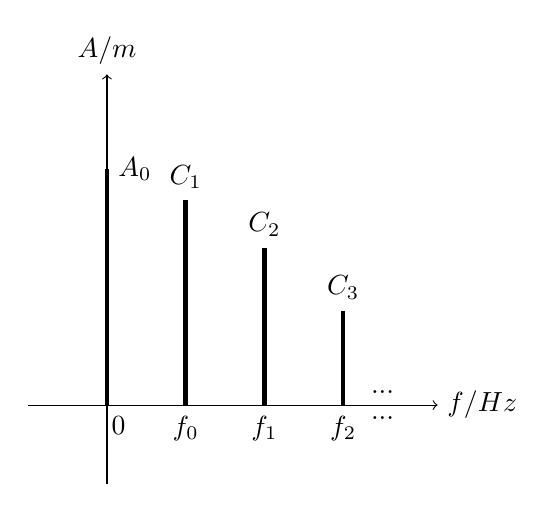
\begin{tikzpicture}
            \draw[->] (-1,0) -- (4.2,0) node[right] {$f/Hz$};
            \draw[->] (0,-1) -- (0,4.2) node[above] {$A/m$};
            \draw[ultra thick, black] (0,0) node[below] {$\;\;\;0$} -- (0,3) node[right] {$A_0$};
            \draw[ultra thick, black] (1,0) node[below] {$f_0$} -- (1,2.6) node[above] {$C_1$};
            \draw[ultra thick, black] (2,0) node[below] {$f_1$} -- (2,2.0) node[above] {$C_2$};
            \draw[ultra thick, black] (3,0) node[below] {$f_2$} -- (3,1.2) node[above] {$C_3$};
            \draw[ultra thick, black] (3.5,0) node[below] {$...$} -- (3.5,0) node[above] {$...$};
        \end{tikzpicture}
    \end{center}
    In which the vertical plots are the spectral lines
    \begin{center}
        $\rightarrow\;$\text{analysis} $\rightarrow$\\
        $\text{Time Domain} \Longleftrightarrow \text{Frequency Domain}$\\
        $\leftarrow$ \text{syntheses}$\;\leftarrow$
    \end{center}

    \subsubsection{Benefits of spectrum}
    \begin{enumerate}
        \item Often time-waveforms are very complicated while spectrun is more straight forward
        \item We can compress data by only storing the important frequencies, shrinking file size (mp3)
        \item Understanding the properties of the signal is often insightful on how to process item
        \begin{itemize}
            \item Think of audio processing, mp3 is a format which removes all frequencies sampled beyond human's limits, also shrinking the file size
            \item We can remove noise
        \end{itemize}
        \item Often easy to see how system affect a signal by determining what-happens to the signal spectrum as it is transmitted through the system
        \begin{itemize}
            \item A radio receiver uses a susem called filler that filters out all frequencies in the received radio wave other than the frequeny of the channel we choosed
        \end{itemize}
    \end{enumerate}
    \subsubsection{Fourier integral}
    For any periodic signal we might need to go beyond just harmonic signals:
    \begin{align}
        x(t) &= \int_{0}^{\infty} A(f)cos(2\pi ft) + B(f)sin(2\pi ft)df\\
        \text{where:\;}\nonumber\\
        A(\omega) &= \frac{1}{\pi} \int_{-\infty}^{\infty} x(t)cos(2\pi ft)dt\\
        B(\omega) &= \frac{1}{\pi} \int_{-\infty}^{\infty} x(t)cos(2\pi ft)dt
    \end{align}
    \subsubsection{Limitations}
    \begin{enumerate}
        \item Arbitrary continuous functions cannot be represented in practice and cannot be stored in computer
        \item The involved integrals cannot be computed in general
    \end{enumerate}
    \subsection{Fourier Transform summary}
    Let $x(t) = x(t + T_0)$ be a periodic signal with period $T_0$, then there exist coefficients $\{A_k\}_{k = 0}^{\infty},\; \{B_k\}_{k = 0}^{\infty}$ such that
    \begin{align}
        x(t) &= \frac{A_0}{2} + \sum_{k=0}^{\infty}\left( A_k cos(2 \pi f_0 k t) + B_k sin(2 \pi f_0 k t)\right), \forall t\\
        A_0 &= \frac{2}{T_0} \int_{-0.5T_0}^{0.5T_0} x(t)dt\\
        A_k &= \frac{2}{T_0} \int_{-0.5T_0}^{0.5T_0} x(t)cos(2\pi kt)dt\\
        B_k &= \frac{2}{T_0} \int_{-0.5T_0}^{0.5T_0} x(t)sin(2\pi kt)dt\\
        &or \nonumber\\
        s(t) &= \frac{A_0}{2} \sum_{k=1}^{\infty} C_k cos(2 \pi f_0t + \phi_k)\\
        &where \nonumber\\
        C_k &= \sqrt{A_k^2 + B_k^2} and \phi_k = tan^{-1}(\frac{B}{A})
    \end{align}
    A spectrum of a periodic signal is the collection of amplitude, 
    frequency and phase information that allows us to represent the signal as a linear combination
    $A_0$ is the DC part of the signal
    Think of the integral as a Riemannian sum, that is, 
    the average of signal over a period

    \subsection{Complex number involved in fourier transform}

    Complex number are an elegant way of expressing rotations, something periodic.

    \begin{align}
        Euler's\;&Formula \nonumber\\
        &R(cos(\theta) + i sin(\theta)) \;(or Rcis(\theta)) \equiv Re^{i\theta}\\\nonumber
    \end{align}

    Adding two complex number

    \begin{align}
        z &= a + bi\\
        z_1 &= a_1 + b_1i\\
        z + z_1 &= a + a_1 + b + b_1i
    \end{align}

    We can easily understand the concept of multiplication and division using Euler's formula

    \begin{align}
        z &= R e^{i\theta}\\
        z_1 &= R_1 e^{i\theta_1}\\
        z \times z_1 &= R \times R_1 \times e^{i(\theta + \theta_1)}
    \end{align}

    A conjugate of an imaginary number is an symmetric image of itself by the $x$-axis

    \begin{align}
        z &= a + bi\\
        z* &= a - bi\\
        z \times z* &= a^2 + b^2\\
        \Re(z) &= \frac{z + z*}{2}\\
        \Im(z) &= \frac{z - z*}{2i}
    \end{align}

    hence 

    \begin{align}
        cos(\theta) &= \frac{e^{i\theta} + e^{-i\theta}}{2}\\
        sin(\theta) &= \frac{e^{i\theta} - e^{-i\theta}}{2i}\\\nonumber
    \end{align}

    \subsubsection{Complex Exponential Signal}

    We can use the conclusion above to express a signal with an complex exponential signal
    \begin{align}
        z(t) &= Ae^{2 \pi f_0 t + \phi}
    \end{align}
    Where $A$ is the magnitude and $\omega_0 + \phi$ is the angle linearly variating in time 

    We can plot an complex exponential signal spectrum for any given signal by seperating them into real part and imaginary part
    \begin{align}
        let\; x(t) &= 10 + 14 cos(200 \pi t - \frac{\pi}{3}) + 8 cos(500 \pi t + \pi/2)\\
        x(t) &= 10 + 7e^{-\frac{j\pi}{3}} e^{2j\pi(100)t} + 7e^{\frac{j\pi}{3}} e^{-2j\pi(100)t}\\
        &\;\;\;\; + 4e^{\frac{j\pi}{2}} e^{2j\pi(250)t} + 4e^{-\frac{j\pi}{2}} e^{2j\pi(250)t} \nonumber
    \end{align}

    \begin{center}
        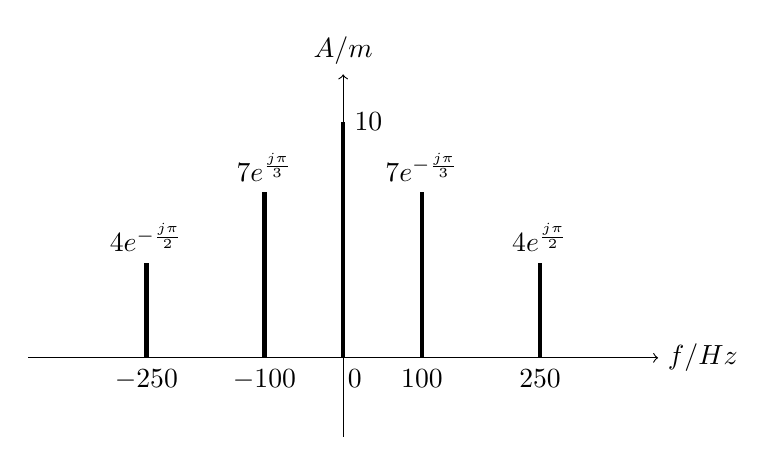
\begin{tikzpicture}
            \draw[->] (-4,0) -- (4,0) node[right] {$f/Hz$};
            \draw[->] (0,-1) -- (0,3.6) node[above] {$A/m$};
            \draw[ultra thick, black] (0,0) node[below] {$\;\;\;0$} -- (0,3) node[right] {$10$};
            \draw[ultra thick, black] (1,0) node[below] {$100$} -- (1,2.1) node[above] {$7e^{-\frac{j\pi}{3}}$};
            \draw[ultra thick, black] (2.5,0) node[below] {$250$} -- (2.5,1.2) node[above] {$4e^{\frac{j\pi}{2}}$};
            \draw[ultra thick, black] (-1,0) node[below] {$-100$} -- (-1,2.1) node[above] {$7e^{\frac{j\pi}{3}}$};
            \draw[ultra thick, black] (-2.5,0) node[below] {$-250$} -- (-2.5,1.2) node[above] {$4e^{-\frac{j\pi}{2}}$};
        \end{tikzpicture}
    \end{center}

    Multiplying something by $i$ jas an effect of rotating that something by 90 degrees. 
    Using euler's formula, we can express any unit-length complex number as $e ^ {(2 \pi i t)}$
    Where $t$ is a real number, if $t$ represents time, 
    and plot the location of the complexnumber at the given time $t$.
    What we will see is a circle being drawn with a frequency of one cycle per second($Hz$).
    We could adjust the speed of the rotation by multiplying a frequency $f$ to the power, 
    which gives us $e ^ {(2 \pi i f t)}$\\

    Can it have negative frequencies? negative frequencies seems pretty abstract at first, 
    but once you start to understand the idea of drawing a circle in the anti-clockwise direction,
    you will soon realise that having negative frequencies simply implies rotating in the clockwise direction.\\

    Multipying the circle by a function $f(t)$ would then suggest wrapping the function around the circle,
    By taking the mean, finding the center of mass of the wrapped signal, at different time t with an integral, we can plot a diagram of the spectrum.
    When it all lined up, there will be an obvious peak. where the center of mass is shiped the farthest away from the signal.\\

    So the complex version of fourier integrals is:

    \begin{align}
        x_k &= \frac{1}{T_0} \int_{0}^{T_0} x(t) e^{-j 2 \pi f_0 kt}
    \end{align}

\section{Discrete Signals}
    \subsection{Aliasing}
    Aliasing in the context of signal processing is simply the same name of two signals. 
    When sampling a signal at a certain frequency, multiple signals at different frequency can produce the same signal
    For, example: $\hat{\omega} + 2\pi l$ and $2\pi l - \hat{\omega}$ are aliases of $\hat{\omega}$
    as they are different discrete times signals defining the same signal values
    \begin{center}
        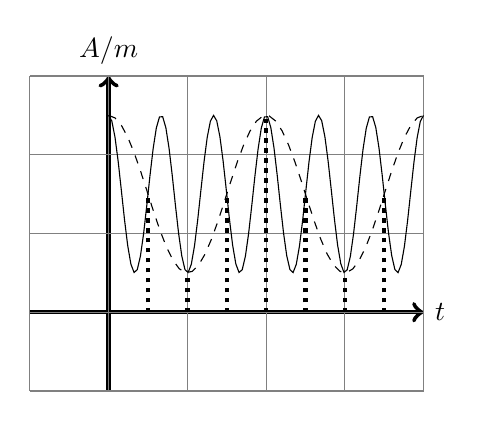
\begin{tikzpicture}
            \draw[->,ultra thick, black] (-1,0) -- (4,0) node[right] {$t$};
            \draw[->,ultra thick, black] (0,-1) -- (0,3) node[above] {$A/m$};
            \draw[gray] (-1,-1) grid (4,3);
            \draw [domain=0:4, samples=50,dashed] plot (\x, {1.5+cos(pi*\x r)});
            \draw [domain=0:4, samples=100] plot (\x, {1.5+cos(pi*\x*3 r)});
            \draw[dotted, ultra thick, black] (0.5,0) -- (0.5,1.5);
            \draw[dotted, ultra thick, black] (1.0,0) -- (1.0,0.5);
            \draw[dotted, ultra thick, black] (1.5,0) -- (1.5,1.5);
            \draw[dotted, ultra thick, black] (2.0,0) -- (2.0,2.5);
            \draw[dotted, ultra thick, black] (2.5,0) -- (2.5,1.5);
            \draw[dotted, ultra thick, black] (3.0,0) -- (3.0,0.5);
            \draw[dotted, ultra thick, black] (3.5,0) -- (3.5,1.5);
        \end{tikzpicture}
    \end{center}
    As you can see from the diagram above, the two signal, both sampled at 2 Hz, 
    produced the same value each sample, but are fundamentally, two different frequencies\\

    The principle alias is the frequency in $[0, \pi]$

    \begin{align}
        \hat{\omega}\; &\hat{\equiv}\; \omega_0 T_s = \frac{\omega_0}{f_s}
    \end{align}

    Fix a discrete sinusioid of discrete-time frequency $\hat{\omega}$, then the frequency $f_0$ of the original continuous
    time sinusoid could have been any of the following:

    \begin{align}
        f_0 = (\frac{\hat{\omega}}{2\pi})f_S \;\text{or}\; f_0 = (\frac{\hat{\omega}}{2\pi})f_S + lf_s \;\text{or}\; f_0 =  lf_s - (\frac{\hat{\omega}}{2\pi})f_s \; where l \in \mathbb{Z}
    \end{align}

    We cannot know which one of them is the true signal, unless we can fix more conditions

    \subsubsection{Sampling sinusoids}

    Take a sample of $x[n] = cos(0.4 \pi n)$, and is equivalent to $x_2[n] = cos(2.4 \pi n)$. An alias corresponding to the principal alias , by convention, is used.
    Once the name is fixed and $f_s$ is known, we canguarantee that the samples came from 
    \begin{align}
        x[n] &=\; cos(0.4 \pi n) \;\text{since}\; \hat{\omega} \in [0,\pi] \\
        \implies \omega_0 &=  \hat{\omega} f_s \in [0,\pi \times f_s]\\
        \implies f_0 &= \frac{f_0}{2\pi} \in [0, \frac{f_s}{2}]
    \end{align}

    If the frequency of the original continuous time signal does not satisfy the condition mentioned above, 
    then the resulting samples are identical to those obtained by sampling a lower frequency signal. So When
    $f_0 \notin [0, \frac{f_s}{2}]$, aliasing occurs.
    
    



   
\end{document}